\chapter{Iterative Bayesian Modelling for Poverty Estimation}

\label{ch:workflow}

This chapter shows how to develop a Bayesian model iteratively to estimate poverty indicators.
The main ideas of Bayesian workflow according to \cite{gelman_bayesian_2020} are summarized in the first section.
The second section presents two plausible alternatives to model skewed, leptokurtic and unimodal variables such as income. GLM models with skewed likelihoods are compared with a data-driven approach similar to \cite{morelli_hierarchical_2021}.
In the third section, the regularized horseshoe prior is explained, which is then used to select variables with adequate predictive power.
The rest of the chapter focuses on the impact of priors on model perfomance.
Section four discusses how to define coefficient and variance priors with the help of prior predictive checks.
In section five, the stratification described chapter \ref{ch:design} is used to redefine the areas and consequently the random effect.
Finally, the last section explores two alternatives to model correlations at the area-level: the LKJ prior and the SAR prior.


\section{An introduction to Bayesian workflow}

The idea of a statistical workflow is not new.
One early example of a statistical workflow can be found in \cite{box_science_1976}.
In the Bayesian context, \cite{gabry_visualization_2019} and \cite{betancourt_towards_2020} have referred to the idea of a Bayesian workflow.
This section summarizes the ideas behind Bayesian workflow as presented by \cite{gelman_bayesian_2020}.

While Bayesian \textit{inference} deals with the formulation and computation of (conditional) probability densities, Bayesian \textit{workflow} consists of three steps: model building, inference and model checking/improvement.
In Bayesian workflow, it is inevitable that a series of models are fit iteratively.
Flawed models are a necessary step towards improving the model and finding models that are useful in practice.
At the same time, model improvement is not limited to finding the best model, but it also lets us better understand the models used; specifically, why they fail or lead to different results under certain conditions.
There are several reasons for considering a workflow and not just plain inference.
Bayesian computation is challenging and it is often necessary to iterate through simpler and alternative models, sometimes using faster but less precise approximation algorithms.
Moreover, it might not be clear ahead of time which model is adequate and how it can be modified or extended.
The relation between fitted models and data can be best understood by comparing inferences from different models.
For example, it is possible to gain valuable insights by comparing a model to simpler or more complex models.
Finally, there is uncertainty associated with model choice, as different models might lead to diverging but realistic results for the same application.

The graphical representation of the workflow is included in Figure \ref{fig:gelman_wf}.
The workflow contains many steps, but the authors emphasize that there are some steps that might be skipped or changed depending on the data and the use case.
For this reason, \cite{gelman_bayesian_2020} argue that a workflow is more general than an example, but less clearly specified than a methodology.
While the exact steps are likely to vary depending on the specific application, a workflow provides a framework to develop statistical models.
Note that this workflow is mostly focused on data modeling.
Other steps such as data collection are not taken into account.

\begin{figure}
    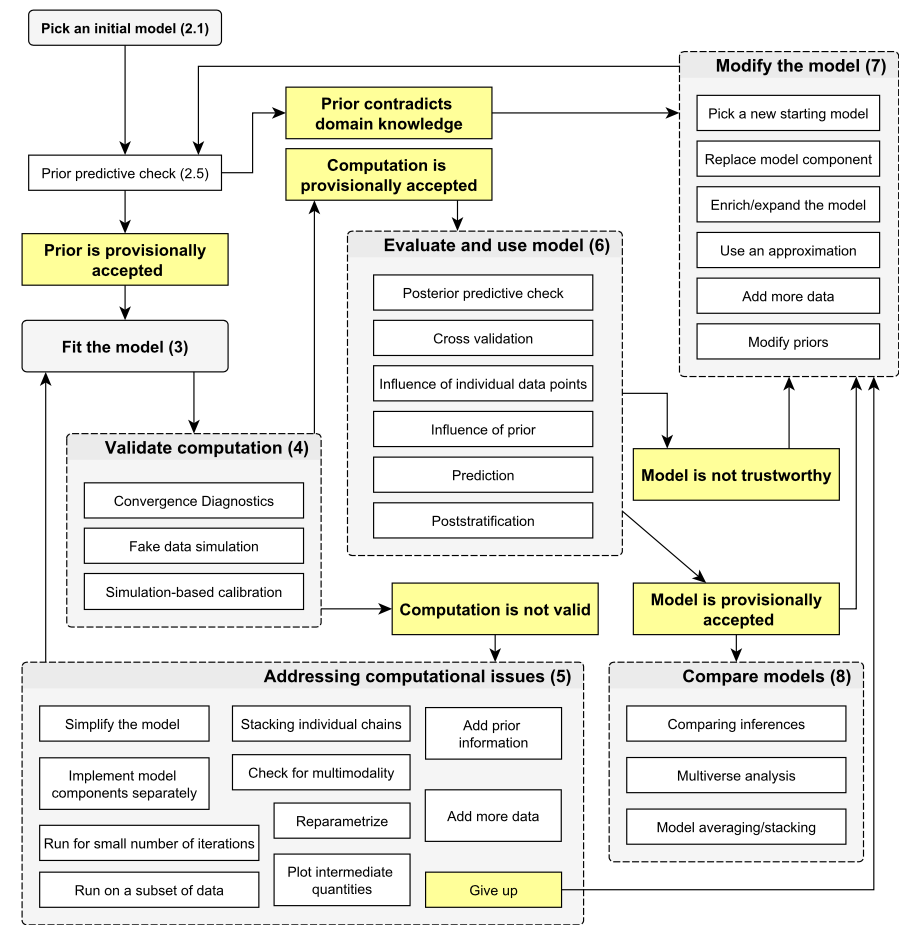
\includegraphics[width=16cm]{./graphics/workflow}
    \caption{Workflow from Gelman et al. (2020).}
    \label{fig:gelman_wf}
\end{figure}


An exhaustive discussion of the whole workflow is beyond the scope of this paper.
Instead, the focus is on how the ideas in \cite{gelman_bayesian_2020} can be applied to the estimation of poverty indicators in the small area estimation context.
Due to the non-linear nature of the workflow, the sections and subsections in the current chapter are not strictly named after single steps of the workflow.
On the contrary, each section in this chapter reflect specific aspects of a model that are investigated separately.
However, throughout the rest of the paper there are explicit references to the corresponding step and an explanation of why it is necessary at a given stage.
For completeness, the rest of this section summarizes the seven workflow steps in \cite{gelman_bayesian_2020} that are also represented in Figure \ref{fig:gelman_wf}.

\subsection{Step 1: pick an initial model}

Usually, the starting point is to adapt an idea that already exists in the literature.
This adaptation can be done in different ways: (i) start with a simple model and add layers of complexity, (ii) simplify a complex model, so that it is more understandable or easier to fit while still delivering a similar performance, (iii) consider different starting models with diverging assumptions and follow multiple paths.
Bayesian models are highly modular, as priors and likelihood can be replaced with other distributions if necessary.
Moreover, there is flexibility regarding how parameter priors interact with each other, which allows for a high degree of model complexity.

%(HERE? )Prior predictive checks are a valuable tool when building a model, because it allows to refine the model without fitting the data multiple times.
%This is especially important when the priors should regularize the model to avoid extreme predictions.
%Additionally, fully generative model?

For example, in this paper, one initial model is the HB model by \cite{molina_small_2014} with its extensions in \cite{morelli_hierarchical_2021}, where the effect of different likelihoods for log-shift transformed income was explored.
The $t$-distribution provides the best performance over many different scenarios.
However, in \cite{morelli_hierarchical_2021} the shift parameter was found through a heuristic whereas
the initial model in the present paper does full inference on the shift parameter from the start.
Additionally, an alternative group of initial models that use skewed likelihoods instead of transformations will be considered in section \ref{ch:skewed_likelihoods}.


\subsection{Step 2: fit the model}

Appendix \ref{ch:computation} discusses the two most common Bayesian estimation approaches: MCMC and variational inference.
When fitting a model, the user is confronted with decisions on which algorithm to run and under which conditions.
To make an adequate choice, it is necessary to be aware of the modelling stage.
MCMC provides the most exact approximation, which becomes more robust with more samples and more chains.
However, if a model was just modified or the user is at an early stage of model development, it is not efficient to fit the model the most exact algorithms and a high number of samples with multiple chain.
Instead, the fit of a bad model should fail fast, as computational issues usually indicate a deeper problem in the model.
Such problems can already be clear with just two Markov chains and a drastically lower number of samples than what would be chosen for the final model.
Even a check with an approximate method such as variational inference might be enough to notice problems with the model, while being drastically faster than MCMC.
In this paper, variational algorithms were often used to do a first fit of the model.
While iterating through the models only two Markov chains were used and, depending on fitting time, the number of iterations was reduced compared to the default 2000 iterations in \code{Stan} \cite{stan_development_team_stan_2021}.


\subsection{Step 3: Validate computation}

After fitting the model it is crucial to check whether the computation results are reliable.
Diagnostics for Bayesian computation methods are discussed in detail in appendix \ref{ch:computation}.
When using an MCMC algorithm such as NUTS, the two main aims are to have no divergences and to have an $\hat R$ lower than 1.01.
All the models presented in this paper fulfill at least these two conditions, unless otherwise specified.
However, adequate diagnostic values are a necessary but not sufficient condition for a reliable model.
To assess model quality, the model has to be fitted to some data set.
The use of real data can be challenging, as there is no way to distinguish modeling issues from computational issues.
This problem can be avoided by using simulated data, ideally from multiple realistic scenarios.
Section \ref{ch:simulations}, already presented three scenarios used in this paper.
A model that can fit fake data, is not necessarily correct, but a model that fails when fitting simulating data will also fail with real data.
This paper deals primarily with prediction, so it is enough if samples from the posterior predictive distribution capture the main characteristics of the data.
There will be less emphasis on correctly recovering other model parameters from the simulated data.

%(Another approach with simulated data is simulation-based calibration.
%First, model parameters are generated from the prior and used to simulate data conditional on these values.
%Then the model is fitted to data and the posterior is compared to the simulated parameters from the priors that were used to generate the data.
%By repeating this procedure, it is possible to check the inference algorithms – the prior should be recovered when performing inference on data sets drawn from the prior.)

\subsection{Step 4: Address computational issues}

A model that leads to computational problems often has some underlying modelling issues.
Usually, it is best to start with a simple model and make it more complex one step at a time, making it easier to determine what part of the model is causing problems.
On the other hand, if the model is already complex and shows signs of computational problems, then it is useful to simplify it step by step until the computation is successful.
For example, in a model with numerous groups of random intercepts or random slopes it makes sense to start with just one group and then add each additional group one step at a time, so as to know whether the estimation is working.
A common source of computational problems is prior choice.
Tightening moderately informative priors can help by pushing the sampler towards certain regions of the parameter space.
However, the priors should be adjusted in line with available knowledge and not only to solve fitting problems.
One such example is discussed in section \ref{ch:log_shift}.

\subsection{Step 5: Evaluate and use the model}

After ensuring that the computation results are reliable, it is necessary to evaluate the quality of the estimated model.
Posterior predictive checks are a useful tool when diagnosing fitting problems to the data.
This can be seen as a safeguard against misspecification.
Moreover, such checks might reveal which aspects of the data are not captured well by the model.
Cross-validation is an alternative to posterior predictive checks and has the advantage that part of the data is left out of the fitting process.
Thus, it is less optimistic than posterior predictive checks, which uses the data for both model fitting and evaluation.
While refittig a model multiple times to do cross-validation can be computationally expensive, there are efficients approximations such as PSIS-LOO \citep{vehtari_practical_2017}.
To check how informative the data is with respect to a parameter, one can compare the standard deviation of prior and posterior parameters. A higher shrinkage in uncertainty indicates that the data is more informative.
If the model is good enough it can be used in an applied setting.
In the small area estimation context, this means generating predictions from the model and calculating poverty indicators.

\subsection{Step 6: Modify the model}

Bayesian statistics provides a modular approach in which models can be expanded or reduced in response to new data or failures to fit the model to the data.
This is usually done by changing certain aspects of the prior distribution.
The prior determines what kind of available information is integrated into the model and acts as a constraint on the fitting procedure.
There are various levels of priors from completely non-informative to highly informative.
However, the way prior information acts on this information depends on the type of parameter.
Parameters controlling central quantities like a mean are less sensitive to weak priors than scale parameters such as variance.
In turn, scale parameters are less sensitive to weak priors than shape parameters, which control the tails of a distribution (e.g., the degrees of freedom in a $t$-distribution).
When expanding the model with additional parameters (e.g., introducing random intercepts or random slopes), it should be considered whether the priors should be tightened to stabilize the estimates, as the amount of data has not changed.
Nevertheless, the priors should not be tightened beyond a range compatible with prior information.
Note that even if a model is trustworthy, it can still make sense to modify it, e.g., because it is an intermediate model that leads to a more complex model.

\subsection{Step 7: Compare models}

Models are fitted many times, for multiple reasons.
It might be easier to start with simple models, before getting to a more complex model. There are often bugs in the code and in the models.
A model might be well-specified, but it could be improved by being expanded.
The priors might only be placeholders, which will be replaced at a later stage.
Moreover, multiple models might provide acceptable results.
Here, model comparison plays an important role.

Comparing different models is always tied to a certain degree of uncertainty.
Instead of choosing the model with the best cross-validation results, using model stacking can give an insight into model differences.
Stacking combines inferences using a weighting that minimizes cross-validation error, as discussed in section \ref{ch:bayesian_evaluation}.
At the same time, care must be taken when comparing a large number of models to reduce the risk of overfitting.
Therefore, it is useful to select only a couple of models at each stage of the workflow for a comparison.

\section{Approaches to modelling income}
\label{ch:initial}
This section compares two different categories of initial models, which corresponds to the first step of the workflow in \cite{gelman_bayesian_2020}.
The first one is an extension of model \ref{eq:mod_hb} from \cite{morelli_hierarchical_2021} that does full Bayesian inference on the shift parameter of the log-shift transform.
The second category includes a series of skewed likelihoods, which are tested against the simulation scenarios from section \ref{ch:simulations} through posterior predictive tests.
At the end of this section, there is a short discussion on the adequacy of each type of model when dealing with unimodal, skewed, leptokurtic data.

\subsection{Alternative 1: Data-driven transformations}
\label{ch:log_shift}

As discussed by \cite{rojas_perilla_data_2020}, data-driven transformations can change the distribution shape of the dependent variable so that it is more convenient to use simple methods such as a linear mixed model with a Gaussian error term.
While \cite{rojas_perilla_data_2020} includes a discussion of multiple data-driven transformations such as the Box-Cox or the Yeo-Johnson, the focus here lies on the log-shift transform, as it is the closest to the conceptually simple logarithmic transform.
This section starts with a general discussion of the log-shift transform and then shows how to include the transform in the Bayesian model.

\subsubsection{Log-shift transformation and skewness}
A common transformation for income in economic applications is the natural logarithm. However, there might still be some skewness left, which is exacerbated by very low incomes.
If there are a lot of units with incomes between zero and one, there will likely be a long tail to the left side of the transformed distribution.
As \cite{rojas_perilla_data_2020} point out, it is possible to add a fixed term $s$ inside the logarithm so that $y+s \ge 1$ to avoid problems when $0 \le y \le 1$,
but the transformed variable might still be highly skewed.
Moreover, log-income is usually heavy-tailed.
This is not surprising, as a variable has to be distributed according to a log-normal distribution for its logarithm to be normally distributed.

To bring the dependent variable closer to a normal distribution, \cite{rojas_perilla_data_2020} explore different types of data-driven transformations such as Box-Cox or Yeo-Johnson.
While effective, these transformations are piecewise functions, which adds an additional layer of complexity when backtransforming to the original scale.
Another more simple data-driven transformation described by \cite{rojas_perilla_data_2020} is the log-shift defined as $y^* = \log(y + \lambda)$, where $y$ is the original variable and $\lambda$ is the shift term. Although $s$ and $\lambda$ fulfill similar purposes, they have different meanings: $s$ is a fixed term chosen in advance, whereas $\lambda$ is a parameter to be estimated.
A key advantage is that the backtransformation is straighforward: $y = e^{y^*} - \lambda$.
By adjusting $\lambda$, it is possible to make the transformed variable more symmetric.
However, as \cite{morelli_hierarchical_2021} points out, the transformed variable might still have considerable excess kurtosis, even when it is almost symmetric.
\cite{rojas_perilla_data_2020} point out that minimizing skewness is just one approach to estimating $\lambda$.
One can also aim to minimize the distance (e.g. Kolomogorov-Smirnov or Cramér-von Mises) to another distribution, usually the Gaussian.
Their preferred approach is to maximize the REML of the model under data-transformations.
For the method proposed in this section, it is only necessary to minimize skewness to better fit the symmetric likelihood chosen for the model in the transformed scale.

There is a further question related to dependent variable skewness in the linear mixed model.
\cite{rojas_perilla_data_2020} propose to a pooled skewness measure that weights the skewness of the unit and area-level error according to their variances.
In principle, it is possible that skewness not only affects the unit-level error $\varepsilon_{di}$, but also the area-level error $u_{d}$.
While right-skewness is a common pattern of income at the unit-level (a few individuals/households earn much more than the rest), the picture is less clear at the area-level, as the areas can be defined in very different ways.
For example, if areas are defined as municipalities, there is a certain degree of arbitrariness to geographic boundaries:
although the Mexican states of Guerrero and Baja California have roughly the same area, the former has 81 municipalities while the latter only has six.
Any distribution of $u_d$ will reflect primarily the arbitrary subdivision rather than an underlying economic phenomenon.
Therefore, only the skewness at the unit-level errors is considered in this paper.
The Bayesian model proposed assumes that $u_d$ follows a normal distribution and is therefore symmetric by definition.

\subsubsection{Estimating the shift parameter}
A key question is how to estimate the shift term $\lambda$.
There are two options: estimate it from the data in an empirical Bayes way or do full Bayesian inference.
Both approaches have their advantages and disadvantages.
When estimating $\lambda$ from the data, the aim is to reduce skewness as much as possible.
This can be done by minimizing the absolute empirical skewness of $y^*$, or at least bringing it below a predetermined threshold.
This approach has the advantage that it is straightforward to control the reduction of skewness in $y^*$.
However, the uncertainty of estimating the shift parameter is not taken into account, as the shift parameter is not included into the model.
In practice, the empirical Bayes that minimizes skewness should be in the same range of the full Bayesian estimate, so it can be used as an additional check for the Bayesian model.

Integrating the shift parameter $\lambda$ naively into the model might lead to estimation problems.
Defining the prior directly on $\lambda$ is not straightforward, as each data set might lead to different results and with no further prior constraints the Markov chains might get stuck and not mix well.
As discussed in the previous section, minimizing the skewness of the transformed variable close to zero is likely to improve the performance of a symmetric likelihood distribution.
In the Bayesian context, this can be done by including a very tight prior on skewness centered around zero
\begin{equation*}
    S(y^*) \sim \mathcal N(0, \delta).
\end{equation*}
Here, $\delta > 0$ is a small positive constant and $S$ is skewness defined as
\begin{equation*}
    \displaystyle S(y^*) =  \frac{\frac 1 N \sum^{N}_{i = 0} (y_i^* - \bar y^* )^3}
    {\left[ \frac{1}{N - 1} \sum^{N}_{i = 0} (y_i^* - \bar y^* )^2 \right]^{3/2}},
\end{equation*}
where $y^* = \log(y + \lambda)$ is the transformed dependent variable. Thus, the prior on $S$ indirectly defines a prior on $\lambda$.
While it is not necessary to formulate a prior directly on $\lambda$, it still recommended to define the lower bound of $\lambda$ as $-\min(y)$ in the programming framework as a safety check, to avoid negative values inside the logarithm function.
In practice, the Markov chain steers clear of regions too close to the minimum for $\lambda$ after warmup iterations.



Because of the transformation, the Jacobian of the likelihood is adjusted by the multiplicative factor $(y_{di} + \lambda)^{-1}$, derived in appendix \ref{appendix:jacobian}. Together with the prior on skewness, this leads to a reformulation of model \ref{eq:mod_hb} as follows:
\begin{equation}
    \begin{split}
        p(\log(y_{di} + \lambda) |\boldsymbol \beta, u_d, \sigma_e, \nu)   =        \text{Student}&(\log(y_{di} + \lambda)| \boldsymbol{x'}_{di} \boldsymbol \beta + u_d,\ \sigma_e\ , \nu)\cdot (y_{di} + \lambda)^{-1}, \\
        u_d | \sigma_u & \sim \mathcal N(0, \sigma_u),\ d = 1, ..., D, \\
        \beta_k & \sim \mathcal N(0, 0.5),\ k = 1, ..., K,\\
        \sigma_u & \sim Ga(2, 0.75), \\
        \sigma_e & \sim Ga(2, 0.75), \\
        \nu & \sim Ga(2, 0.1), \\
        S(\log(y + \lambda)) & \sim \mathcal N(0, \delta), ~ \delta > 0\\
    \end{split}
    \label{eq:trafo_hb}
\end{equation}
where $\ d = 1, ..., D,\ i = 1, ..., N_d$. The transformation $\log(y_{di} + \lambda)$ is left explicitly in the model to remind the reader that the prior on skewness directly affects lambda.
The prior parameterization of $\beta_k, \sigma_u$ and $\sigma_e$ are taken from \cite{morelli_hierarchical_2021}. The lack of index for $y$ inside of $S$ reflects that the skewness function $S(\cdot)$ takes into account all the observations of the target variable – independent of the area.

After a log-shift transformation, the regression coefficients can be interpreted as an approximate percentage change in the original scale.
A detailed justification for this interpretation can be found in appendix \ref{appendix:coeff}.
Note that the use of the exponential distribution in the backtransformation together with the heavy-tailed Student's $t$-distribution can lead to very extreme prediction in the backtransformed scale.
Empirically, the percentage of predictions above the dependent variable maximum is between 0.03\% and 0.5\%.
This proportion is very small and should not have a large impact on the poverty indicators, as they depend on the median, which is robust to outliers.
Nevertheless, it can cause problems when examining the samples from the posterior predictive distribution.
Therefore, all samples that are above the data maximum are taken as missing and are imputed.
The imputation procedure is explained in detail in appendix \ref{ch:imputation}.



The hyperparameter $\delta$ controls the deviation from the zero skewness constraint.
Values around $10^{-2}$ worked well in simulation experiments and the posterior values for $S(y^*)$ are usually very close to zero.
Nevertheless, there are two potential problems to be aware of.
If $\delta$ is too small, then skewness might be reduced too much.
This would be equivalent to overfitting the skewness of the training data, which by no means reflects the skewness of out-of-sample data.
However, if $\delta$ is too large, then many unrealistic values for $\lambda$ will be allowed, which might lead to poorly mixing Markov chains with an $\hat R$ higher than the recommended 1.01.
By plotting the posterior density of $S(y^*)$ and using Bayesian diagnostic tools such as posterior checks, it is possible to assess whether $\delta$ is too small or too large.


\begin{figure}[t]
    \centering
    \begin{subfigure}{0.32\linewidth}
        \includegraphics[width=\textwidth]{./graphics/log_shift/bad_skewness}
        \caption{$S(y^*) \sim \mathcal N (0, 0.1)$}
    \end{subfigure}
    \begin{subfigure}{0.32\linewidth}
        \includegraphics[width=\textwidth]{./graphics/log_shift/mid_skewness}
        \caption{$S(y^*) \sim \mathcal N (0, 0.01)$}
    \end{subfigure}
    \begin{subfigure}{0.32\linewidth}
        \includegraphics[width=\textwidth]{./graphics/log_shift/gb2_skewness}
        \caption{$S(y^*) \sim \mathcal N (0, 0.001)$}
    \end{subfigure}

    \caption[Marginal posterior distribution of skewness for different values of $\delta$.]{Marginal posterior distribution of skewness $S(y^*)$ for different values of $\delta$ in the GB2 scenario: 0.1, 0.01 and 0.001. Note the different scaling of the x-axes.}
    \label{fig:bad_skewness}
\end{figure}

Figure \ref{fig:bad_skewness} shows the posterior density plots of $S(y^*)$ for the GB2 scenario.
The other scenarios displayed similar results.
For $\delta = 0.1$, the mode of the posterior is below zero, which indicates that there is a systematic bias towards negative skewness.
This is problematic when using a symmetric likelihood.
On the other extreme, $\delta = 0.001$ produces an extremely tight distribution around zero.
The range of posterior values for $\lambda$ is very small in this specification, which increases the risk of overfitting the training data.
The middle density graph ($\delta = 0.01$) is a compromise between the two extreme scenarios.
The posterior distribution for $S(y^*)$ is clearly centered around zero, but the posterior is not as tight as with $\delta = 0.001$.
The standard deviation of the shift parameter $\lambda$ is around an order of magnitude larger than in the model with the tighter prior, which allows more possible models and prevents overfitting.
Moreover, the elpd$_{\text{loo}}$ has the highest value with the prior $S(y^*) \sim \mathcal N(0, 0.01)$, which indicates that this is the most adequate specification for the skewness.



\subsubsection{Posterior predictive checks with simulated data}
The results from fitting the modified model \ref{eq:trafo_hb} with the log-shift transformation are presented in Figure \ref{fig:ppc_logshift}.
In the first column, the density of the dependent variable is overlaid with the densities from 100 samples from the posterior predictive distribution.
From this first visual check, it is clear that the model is able to fit the log-scale and GB2 scenarios reasonably well.
The Pareto scenario is still quite close, but the predictions from the model are slightly lower than the dependent variable.
This is an indication that the Pareto scenario contains elements that are particularly challenging to capture.


\begin{figure}
    \begin{subfigure}{\textwidth}
        \includegraphics[width=\linewidth]{./graphics/log_shift/logscale_smp_}
        \caption{Log-scale}
    \end{subfigure}
    \newline
    \begin{subfigure}{\textwidth}
        \includegraphics[width=\linewidth]{./graphics/log_shift/gb2_smp_}
        \caption{GB2}
    \end{subfigure}
    \newline
    \begin{subfigure}{\textwidth}
        \includegraphics[width=\linewidth]{./graphics/log_shift/pareto_smp_}
        \caption{Pareto}
    \end{subfigure}
    \caption[Posterior predictive check for the log-shift model with all three simulation scenarios.]{Posterior predictive check for the log-shift model with all three simulation scenarios. \textit{Left:} density of the dependent variable (black) against the  density of a 100 backtransformed predictions (light blue). \textit{Middle:} scatterplot of IQR against median for 1000 samples. \textit{Right:} scatterplot of standard deviation against mean for 1000 samples. In the middle and right columns, the dark point represents the respective values for the dependent variable in the original data set.}
    \label{fig:ppc_logshift}
\end{figure}

The other two columns show two pairs of descriptive statistics as scatterplots: IQR against median and standard deviation against the mean.
The scatterplots also display the respective descriptive statistic value for the dependent variable.
In the log-scale and GB2 scenarios, the median of the simulations is in a similar range to the median of the dependent variable.
In contrast, the predictions from the model have a median that is around 400 units lower than the dependent variable of the Pareto scenario.
This would mean that the simulated poverty lines (ca. 60\% of 11.900) are systematically lower than the poverty line from the data (ca. 60\% of 12.300) – approximately 3\%.
Thus, certain poverty indicators are likely to be underestimated.
On the other hand, all samples from the posterior predictive distribution in the three scenarios are in a plausible range compared to the IQR of the dependent variable.
The mean and the standard deviation are presented as an additional check, but they are somewhat less trustworthy due to their lack of robustness.
In the logscale scenario, both the mean and the standard deviation are captured well, whereas in the GB2 scenario the mean and standard deviation of the predictions are a little lower than the dependent variable.
The standard deviation Pareto scenario is modelled well, but the mean of the dependent variable is higher than the predictions.
A noteworthy pattern is that in all three scenarios there is a positive correlation between the mean and the standard deviation.
Although the probability density for the backtransformation is not available in its analytical form, it is a clear indication that the mean of the implied distribution is coupled to the variance in the backtransformed scale – a pattern also found in distributions like the lognormal.
The next section explores the performance of models with skewed likelihoods.


\section{Models with Skewed Likelihoods}

A natural question raised by the use of a log-shift transform together with a symmetric likelihood is whether it is better to use a skewed distribution for the likelihood instead.
In line with the Bayesian workflow proposed by (GELMAN ET AL. 2020), different initial models were considered.
The following skewed likelihoods were taken into account: gamma with logarithmic link, gamma with
softplus link, lognormal, skew-normal and exponentially modified Gaussian (exGaussian).

Additive vs. Multiplicative.

The results of these alternative models are presented in this chapter.
To estimate the models the package \code{brms} was used.

% PPC: skew-normal
\begin{figure}[t]
    \centering
    \begin{subfigure}{0.29\textwidth}
        \includegraphics[width=\textwidth]{./graphics/skewed_likelihood/skew_normal/logscale_smp}
        \caption{lognormal}
    \end{subfigure}
    \begin{subfigure}{0.29\textwidth}
        \includegraphics[width=\textwidth]{./graphics/skewed_likelihood/skew_normal/gb2_smp}
        \caption{GB2}
    \end{subfigure}
    \begin{subfigure}{0.29\textwidth}
        \includegraphics[width=\textwidth]{./graphics/skewed_likelihood/skew_normal/pareto_smp}
        \caption{Pareto}
    \end{subfigure}
    \label{fig:skewnormal_ppc}
    \caption[Posterior predictive check for skew-normal likelihood]{Posterior predictive check for skew-normal likelihood. The black line is the density plot of the dependent variable for the respective simulation scenario. The blue density plots represent 100 MCMC draws from the posterior predictive distribution.}
\end{figure}
\vspace{-1cm}
% PPC: exGaussian
\begin{figure}[h]
    \centering
    \begin{subfigure}{0.29\textwidth}
        \includegraphics[width=\textwidth]{./graphics/skewed_likelihood/exgaussian/logscale_smp}
        \caption{lognormal}
    \end{subfigure}
    \begin{subfigure}{0.29\textwidth}
        \includegraphics[width=\textwidth]{./graphics/skewed_likelihood/exgaussian/gb2_smp}
        \caption{GB2}
    \end{subfigure}
    \begin{subfigure}{0.29\textwidth}
        \includegraphics[width=\textwidth]{./graphics/skewed_likelihood/exgaussian/pareto_smp}
        \caption{Pareto}
    \end{subfigure}
    \label{fig:exgaussian_ppc}
    \caption[Posterior predictive check for exGaussian likelihood]{Posterior predictive check for exGaussian likelihood. The black line is the density plot of the dependent variable for the respective simulation scenario. The blue density plots represent 100 MCMC draws from the posterior predictive distribution. Note that the Markov chains have not mixed well in the lognormal and GB2 scenarios.}
\end{figure}

\begin{figure}[t]
    \centering
    \begin{subfigure}{0.29\textwidth}
        \includegraphics[width=\textwidth]{./graphics/skewed_likelihood/gamma_log/logscale_smp}
        \caption{lognormal}
    \end{subfigure}
    \begin{subfigure}{0.29\textwidth}
        \includegraphics[width=\textwidth]{./graphics/skewed_likelihood/gamma_log/gb2_smp}
        \caption{GB2}
    \end{subfigure}
    \begin{subfigure}{0.29\textwidth}
        \includegraphics[width=\textwidth]{./graphics/skewed_likelihood/gamma_log/pareto_smp}
        \caption{Pareto}
    \end{subfigure}
    \label{fig:gamma_ppc}
    \caption[Posterior predictive check for gamma likelihood]{Posterior predictive check for gamma likelihood with logarithmic link. The black line is the density plot of the dependent variable for the respective simulation scenario. The blue density plots represent 100 MCMC draws from the posterior predictive distribution.}
\end{figure}

\begin{figure}[h]
    \centering
    \begin{subfigure}{0.29\textwidth}
        \includegraphics[width=\textwidth]{./graphics/skewed_likelihood/lognormal/logscale_smp}
        \caption{lognormal}
    \end{subfigure}
    \begin{subfigure}{0.29\textwidth}
        \includegraphics[width=\textwidth]{./graphics/skewed_likelihood/lognormal/gb2_smp}
        \caption{GB2}
    \end{subfigure}
    \begin{subfigure}{0.29\textwidth}
        \includegraphics[width=\textwidth]{./graphics/skewed_likelihood/lognormal/pareto_smp}
        \caption{Pareto}
    \end{subfigure}
    \label{fig:lognormal_ppc}
    \caption[Posterior predictive check for lognormal likelihood]{Posterior predictive check for lognormal likelihood. The black line is the density plot of the dependent variable for the respective simulation scenario. The blue density plots represent 100 MCMC draws from the posterior predictive distribution.}
\end{figure}


Some of this likelihoods proved to be very poor fits.
The skew-normal likelihood (Figure \ref{fig:skewnormal_ppc})captures well the main characteristics of the GB2 scenario. On the other hand, it is not adequate for the logscale scenario, which is characterized by a much higher skewness.
This is due to the limitations of the skew-normal distribution, as it has a maximum skewness of $\pm 1$.
Moreover, in this scenario the model produces some negative predictions.
In the Pareto scenario, the model only converged for the version with some out-of-sample areas.
This indicates that the model might need to be reparametrized and the priors adjusted for it to work properly.
However, because this likelihood was already shown to be unreliable for the logscale scenario, the model with a skew-normal likelihood is not further developed.

The exGaussian scenario (Figure \ref{fig:exgaussian_ppc})produces negative predictions in some scenarios and it is not able to capture the main features of the distributions.
While the exGaussian does a good job in the Pareto scenario, it fails on the other scenarios.
In figure Xa and Xb, it can be seen that the algorithm does not converge, with two different posterior predictive as a result.
Placing a more restrictive prior on the coefficients did not alleviate the convergence problem.
However, none of these two distributions adequately captures the main features of the dependent variable in the logscale and GB2 scenarios.
Therefore, this version of the likelihood was also discarded.


The gamma likelihood with a logarithmic link (Figure \ref{fig:lognormal_ppc}) performs quite well on all three scenarios.
Only in the GB2 scenario the posterior predictive draws are flatter than the dependent variable.
Despite its good performance, this model has two drawbacks when fitted to the survey data from Mexico.
First, it takes longer to fit than the log-shifted model presented in this paper, which is likely to be a consequence of the long tails of the distribution.
Second, it is highly dependent on the lowest values.
While in a real income survey there are observations quite close to zero, in the simulation scenarios the minimimum values tend to be somewhat higher.
Due to the non-linear exponential transformation it becomes highly dependent on where exactly the distribution is.
A gamma likelihood with a softplus link function (not shown) produced extremely small predictions, far away from the original order of magnitude and was therefore not further taken into consideration.
Note that the gamma likelihood with a softplus link, as well as the skew-normal and exGaussian distribution, allow for an additive model.
In contrast, distributions that use a log link assume a multiplicative model.

An additional check is provided by a lognormal likelihood (Figure \ref{fig:lognormal_ppc}), which performs well in all three scenarios according to the posterior predictive check.
Nevertheless, the logarithm of a lognormal variable should be normally distributed, which is rarely the case for income data.
Therefore, it is not deemed to be a viable alternative.
\begin{figure}[t]
    \centering
    \begin{subfigure}{0.32\textwidth}
        \includegraphics[width=\textwidth]{./graphics/skewed_likelihood/gamma_log/2d_logscale_smp}
        \caption{logscale}
    \end{subfigure}
    \begin{subfigure}{0.32\textwidth}
        \includegraphics[width=\textwidth]{./graphics/skewed_likelihood/gamma_log/2d_gb2_smp}
        \caption{GB2}
    \end{subfigure}
    \begin{subfigure}{0.32\textwidth}
        \includegraphics[width=\textwidth]{./graphics/skewed_likelihood/gamma_log/2d_pareto_smp}
        \caption{Pareto}
    \end{subfigure}
    \label{fig:gamma_2d}
    \caption[Posterior predictive check with test statistics for gamma likelihood]{Posterior predictive check with test statistics for gamma likelihood with logarithmic link for the logscale, GB2 and Pareto scenarios. The top row shows the meand and the standard deviation, the middle row the median and the IQR and the bottom row the 10\% and 90\% quantiles. The black dot represents the value for the dependent variable, while each one of the blue dots represents the respective summary statistic calculated for each one of the 2000 draws from the Markov chain.}
\end{figure}

As the gamma likelihood with a logarithmic link provided the best fit among the skewed distributions, additional posterior predictive checks are shown in Figure \ref{fig:gamma_2d}.
The two main parameters fitted in a gamma likelihood are the shape and the scale, which directly impact the expected value an the variance.
Thus, it is not suprising that this model performed well in capturing the mean and the standard deviation (top row).
Note the correlation between mean and standard deviation, due to the fact that the coefficient of variation ($\mu / \sigma^2$) is always equal to the shape parameter of the gamma distribution.
The second and third rows of Figure \ref{fig:gamma_2d} uncover more details on the fitting process, because summary statistics such as quantiles are ancillary do not depend directly on the distribution parameters.
In the logscale scenario, which is multiplicative, the model does a good job in capturing the median, the IQR, as well as the 10\% and 90\% quantiles.
In the other two scenarios, the data median is represented well only in the GB2 scenario.
In the Pareto case, the median from the data is somewhat higher than in most of the Monte Carlo simulations.
The estimates for the other test statistics (IQR, 10\% and 90\% quantiles) diverge between the data and the simulations from the posterior predictive distribution.
The 90\% quantile in the dependent variable is lower than in the simulated estimates.
On the other hand, the 10\% quantile is higher than most Monte Carlo simulations.
This shows the model has some trouble with regions further away from the median, which is especially clear in the IQR that is larger in the simulations than in the dependent variables.
The fat right tail in the simulations can also be seen in Figure \ref{fig:gamma_ppc}.
When estimating FGT estimators, it is less relevant whether quantiles above the median can be approximated well, as all observations above 60\% of the median are ignored.
Therefore, it is most important to estimate the median accurately and this is provided by the gamma likelihood with log link.

There are other skewed distributions, where the mode is equal to the minimum.
Some examples include the exponential, the Pareto the chi-squared and the half-normal distributions.
Both the exponential and the chi-squared are special cases of the gamma distribution, which makes them less flexible as likelihood than using a plain gamma distribution.
The half normal has very thin tails and a very low skewness that does not correspond with the long tails observed empirically in income data.

While the main model used in this paper uses a different approach, this does not mean that the use of skewed likelihoods is wrong.
The most promising likelihood was the gamma distribution with a log link.
With this likelihood, it would be possible to avoid very extreme predictions when backtransforming the simulations from the posterior predictive distribution.
However, the heavy right tail might lead to a long model estimation time.
The skew-normal likelihood does not seem to be able to capture the skewness of typical income data, due to its limited maximum skewness.
The exGaussian distribution might be more adequate in this context, but this question is beyond the scope of this paper.



\subsection{Initial model comparison}

In principle, it is possible to keep developing the two alternative models in parallel and then compare them at the end of the workflow, but this implies exploring additional dimension of complexity in the model space.
Therefore, one of both alternatives should be chosen based on the flexibility and limitations of each approach.

The log-shift scenario has two main disadvantages.
By using a log-shift transformation, the user does not exactly know the analytical form of the density in the backtransformed scale.
Moreover, the medians of the posterior predicitve samples in the Pareto scenario are relatively close to the data, but still systematically lower.
Another problem is represented by the very extreme predictions that can arise due to backtransforming samples from the heavy-tailed Student's $t$-distribution.

With respect to the skewed likelihoods, two similar distributions performed well in all three scenarios: the lognormal and the gamma with a log link.
However, these two distribution have theoretical limitations.
On the one hand, the logarithm of a lognormal variable has to be normally distributed, which is rarely the case for income data.
For this reason, it is not deemed to be a realistic alternative.
On the other hand, a gamma distribution has a constant coefficient of variation, which depends on the shape parameter.
Additionally, the logarithm of a gamma distribution is either left-skewed or symmetric, which might not necessarily be realistic for income data.

Whereas the gamma and lognormal distributions only have two parameters (shape/rate or mean/variance, respectively), the main advantage of the log-shift model \ref{eq:trafo_hb} is that it offers more flexibility due to the additional parameters.
The Student's $t$-distribution is not only parametrized in terms of mean and scale, but also of degrees of freedom.
Besides, the log-shift distribution adds another parameter $\lambda$ to the likelihood through the transformed dependent variable.
This flexibility does not come at a high cost of interpretability that characterizes more complex distributions.
While the less than ideal performance in the Pareto scenario is problematic, there are two factors which should be considered.
Firstly, although the prior parametrization was taken mostly from \cite{morelli_hierarchical_2021},
this can be improved through the use of prior predictive checks (see chapter \ref{ch:coef_var_spec}).
Secondly, in this scenario the degrees of freedom were below two, which is not ideal, due to the fact that the Student's $t$-distribution has an infinite variance for $\nu \le 2$ and an undefined variance for $\nu \le 1$.
This extreme behavior might cause problems in the Pareto scenario.
There are two simple solutions to this problem.
Either $\nu$ is set to a constant (e.g., a value between 2 and 3) when the posterior of $\nu$ is clearly below 2, or the model is reparametrized so that $\nu$ does not take values below zero.


In light of this discussion, the log-shift model \ref{eq:trafo_hb} has been chosen for the rest of this paper, as it provides a good balance between interpretability, ease of parametrization and flexibility.
Additionally, it extends the literature on data-driven transformation in the line of \cite{rojas_perilla_data_2020} to the Bayesian paradigm.
This does not mean that the use of skewed likelihoods is an inferior approach, only that its use with income data is left for future research.
A feature of the gamma likelihood that can be useful is that its mean can be parametrized in the original scale even when using a log link as done in the \code{brms} package.
This is particularly relevant, if benchmarking \citep{pfeffermann_new_2013} should be included as a module in the Bayesian model.
For example, a somewhat narrow prior can be placed on the mean of all domain estimates so that it roughly matches the benchmarking mean based on the direct estimates.
The integration of benchmarking into the model is not further considered in this paper.


\section{Specification of coefficient and variance priors}

After deciding that the likelihood should include a shift term and selecting the subset of covariates with the best predictive power, the next step will focus on the plausibility of the priors introduced in model XY from (Morelli 2021).

Section XY showed that even with a shift term in the logarithmic transformation, the coefficients can be interpreted as the approximate percentage change of the dependent variable in the original scale.
This approximation holds mostly for coefficients between -0.3 and 0.3.
However, a change of around 30\% in the original scale for each additional unit is itself very high and this fact can be included in the prior distribution.
Moreover, note that through the use of the logarithmic transform the covariates have a multiplicative effect on the original scale.
Thus, somewhat large coefficients in the logarithmic scale can have a huge impact when backtransforming to the original scale.

There are two main ways to define priors on coefficients, either by assuming that the coefficient priors are independent or by using a joint prior such as a horseshoe prior.
In this section, two independent priors are proposed for the coefficients, which are then compared with the joint prior (ja, wirklich?). However, in this case there are relatively speaking few variables and a horseshoe prior might make more sense with more variables (?)
The comparison will be done with prior predictive checks based on the variables from the selected variables of the MCS survey.
For the independent priors, two different types of distribution can be considered, either a normal distribution or a heavy-tailed distribution such as the Student's $t$ with 3 degrees of freedom.
In this case, a distribution with heavier tails is not as desirable, because even if most of the probability mass is contained in the interval between -0.3 and 0.3, the prior would allow more extreme values.
This can be avoided by choosing a Gaussian distribution, which does not have as much probability mass on extreme values.
The coefficient prior is parametrized to have a mean of zero and a standard deviation of 0.2, which implies that the 5\% and 95\% quantiles are around -0.3 and 0.3 respectively.

Another key element of the models is how the priors are defined for the standard deviations at the unit-level ($\sigma_e$) and area-level ($\sigma_u$).
As the likelihood is a generalized Student's $t$-distribution, the parameter $\sigma_e$ cannot be interpreted directly as the standard deviation of the distribution.
Given a random variable $Y$ that follows this distribution, the variance is given by $Var(Y) = \sigma_e^2 \frac{\nu}{\nu - 2}$.
To reason more easily about the unit-level variancem a new parameter $\sigma = \sqrt{Var(Y)}$ is introduced so that $\sigma_e = \sigma \sqrt{\frac{\nu - 2}{\nu}}$.
In line with model XY, the distribution $\sigma \sim Ga(2, 0.75)$ is still used.
The effect of the prior on $\sigma$ and $\sigma_u$ will be analyzed as part of the prior predictive checks.

For the prior predictive checks, the shift term is dropped. The shift term depends on the dependent variable so it is not possible to sample from its prior distribution.
Besides, it amounts to an additive constant in the backtransformed scale ($e^{y^*} - \lambda$). The impact of the exponential function is therefore much larger than the effect of the shift term $\lambda$.
The range of Mexican income data is in the tens of thousands, which is also captured in the simulation scenarios.
Therefore, the prior predictive simulations should not be above 12 in the logarithmic scale (which corresponds to around 160000 pesos in the original scale).
Conversely, as the original data has almost not observations below 1, the values in the logarithmic scale should not go far below zero.
Finally, note that the degrees of freedom in the Student's $t$-distribution can lead to very extreme simulations when $\nu$ is low.
As a consequence, the prior for $\nu$ is changed to $Ga(2, 1)$ for the prior predictive check only to get lower values.
The minimum value for $\nu$ is 2, so that the variance of the distribution is still finite.
The assumption here is that if the prior predictive simulations are not too extreme for low degrees of freedom, they will also be in a reasonable range for high values of $\nu$, for which the likelihood has thinner tails.

The results for the starting model in XY can be seen in Figure XY.
The scale is much larger for the prior predictive draws, which is especially problematic in the logarithmic scale.

The priors for the variance parameters are tightened to $Ga(2, 10)$.
This yields more realistic results.

The results for prior predictive checks for even variances can be found in appendix XY.

\begin{figure}
    \includegraphics[width=\textwidth]{./graphics/prior_predictive_checks/prior_check_pareto_start}
    \label{fig:ppc_start}
    \caption{Prior predictive check.}
\end{figure}

\begin{figure}
    \includegraphics[width=\textwidth]{./graphics/prior_predictive_checks/prior_check_pareto_tight}
    \label{fig:ppc_tight}
    \caption{Prior predictive check.}
\end{figure}





\section{Variable selection}
\label{ch:varsel}
A key step in specifying the model is deciding which variables to use.
However, this is at the same time one of the more challenging steps.
The ideal solution would be to estimate models with all possible variable combinations and then compare the predictive quality of the models – e.g., through cross-validaton.
However, this solution is not feasible computationally due to the very large number of possible models.
Another common approach is to use shrinkage methods like the Lasso \citep{tibshirani_regression_1996} to determine which variables can be left out without significantly compromising the predictive power of the model.
If a coefficient is shrunk to zero, it is a sign that the respective variable might be removed.
In this section, the regularized horseshoe prior \citep{piironen_sparsity_2017}, which follows a similar shrinkage principle to the Lasso or the ridge, is presented and then used to select relevant variables.
This section shows how priors can be used inside a Bayesian workflow to do variable selection.
The selection is done by comparing the elpd$_{\text{loo}}$ of models with different groups of less meaningful variables removed. An alternative to the horseshoe prior is to use projective prediction approach developed by \cite{piironen_projective_2020}.
Unfortunately, this only works with distributions from the exponential family, which does not include the Student's $t$-distribution used in this paper.
Therefore, the focus lies on the regularized horseshoe prior.

\subsection{Regularized horseshoe prior}

In the Bayesian framework, shrinkage can be best understood in relation to the prior.
The general idea is to have a narrow region of high density around zero that shrinks coefficients,
while at the same time including fat tails to allow some coefficients to deviate from zero over a wider range.
In its most extreme formulation, it corresponds to the spike-and-slab prior introduced originally by \cite{mitchell_bayesian_1988}.
While this prior has a hight theoretical relevance, it can be computationally demanding for a large number of variables and is sensitive to specification details such as slab width.
On the other hand, continuous shrinkage priors provide similar results while also being easier to compute \citep{piironen_sparsity_2017}.
The horseshoe prior \citep{carvalho_horseshoe_2010} is a continuous shrinkage prior with a similar performance to the spike-and-slab prior and can be formulated as follows
\begin{equation}
    \begin{split}
        \theta_j | \lambda_j, \tau & \sim \mathcal N (0, \tau^2\lambda^2_j), \\
        \lambda_j & \sim \mathcal C^+ (0, 1), ~~ j = 1,..., J,
    \end{split}
    \label{eq_hs}
\end{equation}
where $\theta_j$ are the parameters to be shrunk and $\mathcal C^+$ is the half-Cauchy distribution. In a regression setting, $\theta_j$ corresponds to the coefficients $\beta_j$.
This prior is characterized by a global parameter $\tau$ that shrinks all parameters towards zero as $\tau \rightarrow 0$ and a local parameter $\lambda_j$ for each $\theta_j$ that pushes against the global shrinkage.
Due to the extremely heavy tails of $\mathcal C^+(0, 1)$, some $\lambda_j$ will be large enough to counteract even small values of $\tau$.

However, there is no consensus on how to do inference for $\tau$ and parameters far from zero are not shrunk at all.
\cite{piironen_sparsity_2017} address this issues by introducing the regularized horseshoe prior, which is given by
\begin{equation}
    \begin{split}
        \theta_j | \lambda_j, \tau & \sim \mathcal N (0, \tau^2 \tilde \lambda^2_j),
        ~~ \tilde \lambda_j^2 = \displaystyle \frac{c^2 \lambda^2_j}{c^2 + \tau^2 \lambda_j^2}\\
        \lambda_j & \sim \mathcal C^+ (0, 1), ~~ j = 1,..., J,
    \end{split}
\end{equation}
where $c > 0$ is a constant.
If $\tau^2\lambda^2_j \ll c^2$, then $\theta_j$ is shrunk strongly towards zero and $\tilde \lambda^2_j \rightarrow \lambda^2_j$, which approximates the original horseshoe in expression \ref{eq_hs}.
For the case $\tau^2\lambda^2_j \gg c^2$, then $\tilde \lambda^2_j \rightarrow c^2/\tau^2$ and the prior reduces to $\mathcal N(0, c^2)$, which corresponds to a Gaussian slab with variance $c^2$ that regularizes $\theta_j$.
When $c \rightarrow \infty$ the regularizing effect of the prior disappears, just as in the original horseshoe.
Although $c$ can be chosen as a constant, \cite{piironen_sparsity_2017} recommend doing inference with the prior
\begin{equation*}
    c^2 \sim \text{Inv-Gamma}(\alpha, \beta), ~~ \alpha = \nu/2, ~~ \beta = \nu s^2/2,
\end{equation*}
which leads to a Student$(0, s^2, \nu)$ slab for $\theta_j$ far away from zero.
This is desirable as the heavier tails of the Student's $t$ distribution prevent too much probability mass accumulating near zero.

The last parameter in the specification of the regularized horseshoe is $\tau$.
For a linear model, \cite{piironen_sparsity_2017} explore different specifications for $\tau$.
Defining $p_0$ as the prior guess of the number of nonzero variables, the prior for $\tau$ should have most of its mass near
\begin{equation}
    \displaystyle \tau_0 = \frac{p_0}{J-p_0}\frac{\sigma}{\sqrt n},
    \label{eq_tau0}
\end{equation}
where $\sigma$ is the variance of the error term\footnote{In \cite{piironen_sparsity_2017}, the assumed linear model does not have a random intercept. Thus the randomness comes mostly from the unit-level error term $\varepsilon ~ \mathcal N (0, \sigma)$.}.
However, there is no best choice for the prior of $\tau$. The three main options are setting $\tau = \tau_0$, or assuming either $\tau \sim \mathcal C^+(0, \tau_0^2)$ or $\tau \sim \mathcal N^+(0, \tau_0^2)$, where $\mathcal{N^+}$ is the half-normal distribution.
In practice, it is common to set the ratio of relevant and irrelevant parameters, – $p_0/(J - p_0)$ –, and use $\tau = \tau_0$.
In this paper, a ratio of 0.2 is chosen, which assumes that for every 10 irrelevant regressors, there are 2 relevant variables.
Note that the definition of $\tau_0$ in equation \ref{eq_tau0} is derived under the assumption of a Gaussian model.
Therefore, its meaning is only an approximation when using the Student's $t$-distribution.

Certain shrinkage methods like Lasso force certain coefficients to be zero, which provides an easy selection criterion.
However, a disadvantage of the horseshoe is that it does not have an integrated criterion to select variables. There are two possible workarounds for this problem.
First, one could leave out variables whose mean coefficient is below a certain threshold \citep{piironen_sparsity_2017}.
Second, one can leave out variables if a significant portion of the coefficient distribution is in both a positive and a negative area.
To check that the predictive power of the model does not deteriorate by removing variables, PSIS-LOO can be used to compare the full model with the smaller model.

\subsection{Results of variable selection and further considerations}
To avoid implementing the horseshoe prior from scratch, the package \code{brms} was used.
As the package does not provide data-driven transformations, the model is estimated with a simple logarithmic transformation of income and a Student's $t$-likelihood.
While this does not correspond exactly to the log-shift model presented in the previous section, it can be seen as an approximation.
The shift term is unlikely to have a major impact on the predictive power of the regressors.
This can be clearly seen in the backtransformation ($e^\eta - \lambda$, with $\eta$ the linear predictor), where the shift term is just an additive constant shifting $e^\eta$.
The original horseshoe prior does not take into account the grouping of categorical variables.
In this case, if any of the categories has a clear effect on the dependent variable, the whole variable is considered to be relevant.

After estimating the full model with the horseshoe prior, the following variables presented in section \ref{ch:mexican_data} have either very small effects or effects that are not clearly positive or negative: job experience of head of household, gender of head of household, presence of minors under the age of 16, percentage of working household members, percentage of women in household and percentage of literate members of household.
The density plots of the coefficients can be found in Figure \ref{fig:hs_dens} in appendix \ref{appendix:horseshoe_plot}.
A reduced model without these six variables but with the same prior and likelihood specification as the full model was estimated in a second step, but the difference in elpd$_{\text{loo}}$ to the full model is -17.8 with a standard error for the difference of 7.3.
The difference is therefore more than twice as large as its standard error, so it reduces the predictive power of the model.
A second model with only gender of head of household, percentage of women in household and percentage of literate members of household removed is indistinguishable from the full model with an elpd$_{\text{loo}}$ difference of -2.7 and a difference standard error of 4.2.
Therefore, the variables selected in the second model are used for the rest of the paper.

Before moving to the next section, two issues need to be addressed.
First, the effectiveness of the horseshoe prior depends crucially on the number of variables included in the full model.
The shrinkage will be most noticeable with a large number of variables.
Otherwise, the shrinkage from the horseshoe is very similar to placing a prior centered around zero for the coefficients.
In this project, ca. 20 variables were chosen from the survey and census data.
Therefore, the shrinkage of the regularized horseshoe is not much different from the shrinkage of a non-structured prior (e.g., independent normal priors on the regression coefficients).
In any case, this section showed that it is possible to select variables using the horseshoe prior and that its shrinkage properties are particularly useful in high-dimensional data sets.

Finally, finding an adequate subset of variables is a field of active research in the context of Bayesian workflow.
Projective predictive distribution provides a clear selection of variables that keeps the predictive power of the full model, but at the moment of writing only available for the exponential family \citep{piironen_sparsity_2017}.
As the $t$-distribution is one of the likelihoods used in this paper, no projective predicitve methods are used in this paper.
It is very likely that in the near future there will be new tools to do this step of the workflow, especially concerning the projective predictive method to distributions outside the exponential family.


\section{Specification of the random effect}
\label{ch:raneff}
In applications of small area estimation methods, the random effect $u_d$ is usually defined in terms of the domain for which the indicators should be calculated.
For example, \cite{rojas_perilla_data_2020} use a random effect at the municipality level in the model, as the poverty indicators of interest have to be calculated for each municipality.
However, this approach poses two problems.
Firstly, the information contained in the survey design might be overlooked.
There is no guarantee that the random effect is meaningful from the perspective of how the sample was constructed.
Secondly, it might lead to very sparse areas with lots of out-of-sample areas.
In this section, the traditional way of defining the random effect is compared to an approach that approximates the stratification in the survey design as an additional iteration of the model\footnote{The alternative specification of the random effect in this section is included only as an improvement of the model in the Bayesian workflow context. However, there is nothing in the definition of the random effect itself exclusive to  the Bayesian paradigm. The same ideas could also be applied to the frequentist EBP with transformations \citep{rojas_perilla_data_2020}, as it also uses a Monte Carlo approach.}.

Section \ref{ch:design} included a short introduction to the survey design of the data from the Mexican state of Guerrero.
On closer inspection, municipalities play no role whatsoever in the sampling process of the households.
Instead, the population is stratified by federal state, by geographic region (urban or rural) and also by socio-economic indicators taken from the previous census.
Changing the definition of the random intercept does not have any adverse impact on the calculation of FGT indicators.
As the data is at the unit-level and each observation has information on which municipality it belongs to, it is not necessary that the random effect coincides with the municipality.
Predictions for income at the unit-level can be generated from any model as discussed in section \ref{ch:indicators} and the FGT indicator can be calculated simply by using the municipality as a grouping variable.

A major challenge is to find a structure that can be found both in the survey and the census.
While the survey includes a variable that indicates the stratum to which a given observation belongs, this cannot be matched with the stratum contained in the census.
Therefore, the stratification variable in the data cannot be used directly.
However, there are some variables in both the survey and the census that can be used to approximate the stratification procedure.
In addition to the \code{rururb} variable that indicates whether the observation corresponds to a rural or urban area, there are four additional binary variables (Table \ref{tab:disadvantages}), which contain information on disadvantage in areas such as education, health care, housing quality and access to public utilities.
As all five variables are binary, there are $2^5 = 32$ possible combinations.
Each one of these 32 combinations is now considered as a domain that is used to define the varying intercept in the model.\footnote{The strata domains are coded as a binary number with five digits. Each digit represents one variable in the following order: \code{rururb}, \code{ic\_rezedu}, \code{ic\_asalud}, \code{ic\_sbv}, \code{ic\_cv}. For the \code{rururb} variable 1 represents "rural" and 0 "urban". For all the other variables, 1 represents the presence of a disadvantage measured by each indicator as defined in Table \ref{tab:disadvantages}.}
The variable \code{rururb} is no longer used as a regressor in this specification.
This definition of the domain results in sample sizes between 2 and 368 with a median of 37.
No domains are out-of-sample.

The results from PSIS-LOO using model \ref{eq:trafo_coef_var} show that the stratified specification is clearly better. The elpd$_{\text{loo}}$ for this specification is around 34.8 higher than when using  municipalities as the domains.
The standard error for the difference in elpd$_{\text{loo}}$ between both specifications is 12.8, which is around one third of the difference itself.
Even if the models were not substantially different in predictive terms, there is one substantial advantage of using the alternative specification: there are no out-of-sample domains.
This drastically reduces the uncertainty in the predictions for out-of-sample municipalities.
Therefore, the stratified specification of the domain is used in the rest of this paper.

There are some limitations to this approach.
Firstly, the stratified structure is only an approximation.
Secondly, there are still other dimensions that are not taken into account that might still be problematic, e.g., the clustering that stems from structuring the sample process with PSUs.
Thirdly, this is an example that is limited to the data from Mexico.
Other statistical institutes might provide more detailed variables for the strata or none at all and depending on the survey design the approach developed in this section might not even be applicable.
Nevertheless, the main insight from this section is that for unit-level data the random effect does not have to follow the level at which indicators are estimated and that these improvements can be evaluated in a Bayesian workflow.
Looking for alternative specifications for the random effect might lead to better predicitive power and to fewer out-of-sample domains.
\section{Modelling correlations at the area-level}

Until now, the assumption has been that all random effects at the area-level are independent from each other, i.e., $u_d|\sigma_u \sim \mathcal N (0, \sigma_u)$.
However, this assumption seems unplausible.
For example, if the areas are defined as municipalities, it is likely that neighbouring regions have similar characteristics and are therefore correlated.
If on the other hand the areas are the strata considered in the previous section, the 16 strata that correspond to a rural area have more in common with each other than with urban strata.
Here, the independence assumption does not seem realistic either.
In the section, a new prior that captures correlations at the area level is introduced to the model.
The result is then compared to the model that was defined in the previous section.
Thus, the domains are not defined as the municipalities, but as the strata presented in the last section.

There are multiple options to model correlation between areas.
The simpler LKJ prior based on the work by \cite{lewandowski_generating_2009} places a restriction over permissible correlation matrices.
Autoregressive approaches such as IAR, CAR and SAR \citep{chung_bayesian_2020} represent another way of capturing spatial correlation and takes into account how similar or close the different domains are.
Moreover, other priors such as the random walk prior used used in \cite{gao_improving_2021} offers an alternative to modelling dependencies between areas.

The resulting model will be compared with the model that assumes independence from the previous section.
A comparison between all possible priors that capture area correlation is beyond the scope of this paper and left for future research.

\subsection{LKJ prior}

Let $\Sigma$ be a $D \times D$ covariance matrix, so that $u \sim \mathcal{N}(\boldsymbol{0}, \Sigma)$, where $\boldsymbol 0$ and $u$ are $D$-dimensional vectors.
Therefore, the density of $u$ can be written as:
\begin{gather*}
    p(u|\Sigma) = (2\pi)^{-\frac D 2}\det(\Sigma)^{-\frac 1 2} e^{(-\frac 1 2 u'\Sigma^{-1} u)}.
\end{gather*}
The covariance matrix $\Sigma$ can be decomposed as $\Sigma = \text{diag}(\tau)\Omega\text{diag}(\tau)$, where $\tau$ is a $D$-dimensional vector of scale factor, $\text{diag}(\tau)$ is a $D \times D$ matrix with $\tau$ as its main diagonal and $\Omega$ is a $D \times D$ correlation matrix.
Up to this point, the assumption has been that there is only one scale parameter $\sigma_u$ for all area-level effects $u_d$ and this assumption still holds.
Because $\tau_d = \sqrt{\Sigma_{d, d}}$, the decomposition is simplified to $\Sigma = \sigma_u^2 \Omega$.

The standard deviation for the random effect $\sigma_u^2$, already has the prior $Ga(2, 10)$.
However, the correlation between the single random effects is captured by defining a LKJ prior over the correlation matrix $\Omega$:
\begin{gather*}
    \Omega \sim \text{LKJ}(\eta), ~~ \eta \ge 1.
\end{gather*}
The LKJ correlation distribution implies that $p(\Sigma|\eta) \propto \det(\Sigma)^{\eta - 1}$ \citep[Chapter 1.13]{stan_development_team_stan_2021}.
Note that the determinant of $\Sigma$ increases as the correlation between components decreases:
an identity matrix has a determinant of 1, while a correlation matrix consisting only of ones (perfect correlation between components) has a determinant of 0.
For $\eta = 1$, the LKJ prior is a uniform distribution over all possible correlation matrices.
However, due to the fact that the function $f(x) = k^x$ for a fixed $k \in (0, 1)$ does not converge uniformly towards zero as $x \rightarrow \infty$, a higher $\eta$ puts more probability mass on matrices with a higher determinant, i.e., on matrices with a lower correlation between components.\footnote{In practice, it is common to use the Cholesky decomposition of $\Omega$ to avoid numerical issues when estimating the model.
For clarity, the traditional matrix specification is kept in the paper, but note that the decomposition is used in the accompanying code.}

The results from the model comparison can be seen in in Table XY.
The model that allows for correlation between areas has a slightly better performance according to PSIS-LOO than the model with no correlation at all.
However, it is important to remember that elpd$_{\text{LOO}}$ is just an approximation, because PSIS-LOO quantifies predictive power at the unit-level and not at the area-level, whereas the aim of the model is to generate prediction at the area-level.
It is likely that the difference between the predictive power of both specifications would be clearer when using leave-one-group-out cross-validation.
Unfortunately, this is still an area of active research and it is therefore beyond the scope of this paper.
In any case, the slightly better performance of the model with the LKJ priors is taken as a sign that it captures correlations between strata that improve predictions.
Eta parameter?

Figure XY shows four posterior draws for Omega as heatmaps. In the plot, it is possible to see a very clear pattern, that is consistent among draws.



In the current model specification, the random intercept was redifined so that there are no out-of-sample areas.
Nevertheless, the LKJ prior is not as useful when there are out-of-sample regions, as the correlation matrix is assumed to have as many dimensions as in the training set.
In such cases, an autoregressive or a random walk prior on $u_d$ such as in \cite{gao_improving_2021} can be more appropriate, as it does not depend strictly on the dimensions of the correlation matrix.

\begin{figure}
    \begin{subfigure}{\linewidth}
        \centering
        \includegraphics[width=0.85\textwidth]{./graphics/rand_intercept/lkj_corr_plot}
        \caption{LKJ(5) prior}
    \end{subfigure}
    \begin{subfigure}{\linewidth}
        \centering
        \includegraphics[width=0.85\textwidth]{./graphics/rand_intercept/sar_corr_plot}
        \caption{SAR prior}
    \end{subfigure}
    \caption[Correlation matrices for the LKJ and SAR priors.]{Four samples of the posterior correlation matrices for the models with LKJ and SAR priors. The coding of the domains in the axes is explained in section \ref{ch:raneff}.}
    \label{fig:corr_heatmap}
\end{figure}


\subsection{SAR prior}
The simultaneous autoregression (SAR) prior as described in \cite{chung_bayesian_2020} is defined on a precision matrix $\Omega$.
The starting point is the $D\times D$ proximity matrix $W$, which contains information on how close two strata are.
If $w_d, d = 1, ..., D$ is the sum of row $d$ of matrix $M$ ($w_d = \displaystyle \sum_{i = 1}^D w_{di}$), then the $D \times D$ matrix $L$ is defined as $L = \text{diag}\{w_d\}_{d=1}^D$, which is used to calculate the row-normalized matrix $\tilde W = L^{-1}W$.
The SAR prior in the context of model \ref{eq:trafo_coef_var} is then given by
\begin{gather*}
    \Omega(\rho) = (I_D - \rho \tilde W)'(I_D - \rho \tilde W), ~~ \rho \in (-1, 1),\\
    u \sim \mathcal N(\boldsymbol{0}_D, \sigma_u^2 \Omega^{-1}),\\
    \rho \sim \mathcal U(-1, 1)
\end{gather*}
where $\boldsymbol{0}_D$ is a $D$-dimensional zero vector.
As the single strata are coded as a 5-digit binary string (Section \ref{ch:raneff}), the distance matrix $W$ is defined using the Hamming distance.
In short, the Hamming distance takes two strings of the same length and counts how many digits are different, e.g., 00111 and 10100 have a Hamming distance of 3.
This also ensure that the distance of each stratum from itself is 0.
The maximum distance in this case is 5 as each stratum is marked with five binary digits.
Note that when $\rho = 0$ the precision matrix $\Omega$ is equal to the identity matrix, which means that there is not correlation between the domains.
As $\rho$ deviates from 0, the effect of the spatial increases.
The uniform prior is chosen for $\rho$, because it is not straightforward to know which values are likely before fitting the model to the data.
The limits $\rho \in (-1, 1)$ are needed so that $\Omega$ is still positive definite.
The posterior distribution of $\rho$ is left skewed, with 70\% of the probability mass between -1 and 0 and the rest between 0 and 1.

\subsection{Comparison of LKJ and SAR priors}
The main difference with the LKJ prior is that the SAR prior uses actual information on how similar or close the domains are.
In contrast, the LKJ prior is only a prior on the admissible correlation matrices.
The difference becomes clear in Figure \ref{fig:corr_heatmap}, which show four posterior samples of the correlation matrices from the models with the LKJ and SAR priors.
The axes display the respective strata combinations, whose notation as a 5-digit binary string (e.g., 01100) was explained in section .
The correlation matrices produced by the LKJ prior display a completely random pattern with respect to the correlations.
On the othe side, with the SAR prior there is a clear structure in the correlation matrix stemming from the distance matrix $W$.
Even though in Figure \ref{fig:corr_heatmap} the correlation values vary from sample to sample, there is a very clear symmetric visible for each sample, which is related to the way Hamming distance used to define $W$.
The nature of the pattern can be further understood in Figure \ref{fig:corr_density}, which shows the distributions of the correlation values for each one of the sample in Figure \ref{fig:corr_heatmap}.
The LKJ prior does not force any particular correlation pattern on the data, but it guarantees that the distribution of the correlations is roughly equal for each sample.
With an increasing $\eta$, the LKJ prior puts more weight on correlation matrices closer to the identity matrix, which leads to tighter distributions for the correlation values.
On the other hand, there is a much clearer pattern in the densities of the SAR prior specifications.
The spikes in the densities are cause by the Hamming distance, which in the present paper has takes only six values, from 0 to 5.
With continuous distances, the densities would be much smoother.

\begin{figure}
    \begin{subfigure}{0.49\linewidth}
        \includegraphics[width=0.85\textwidth]{./graphics/rand_intercept/lkj_dens_plot}
        \caption{LKJ(5) prior}
    \end{subfigure}
    \begin{subfigure}{0.49\linewidth}
        \includegraphics[width=0.85\textwidth]{./graphics/rand_intercept/sar_dens_plot}
        \caption{SAR prior}
    \end{subfigure}
    \caption[Correlation density for the LKJ and SAR priors]{Correlation density for the four posterior samples of the LKJ and SAR priors shown in Figure \ref{fig:corr_density}. Each sample are displayed in different colors. The correlation in the SAR prior tends to be lower.}
    \label{fig:corr_density}
\end{figure}


The LKJ and SAR specification are compared with the model without domain-level correlation (base model) using PSIS-LOO.
The results are shown in Table \ref{tab:lkj_sar_base}.
The elpd$_{\text{loo}}$ of the SAR model is slightly worse than the base model (-0.07), but the standard error of the difference (second column) is more than three times the estimated elpd$_{\text{loo}}$ difference itself (0.24).
According to PSIS-LOO, the base and SAR models are undistinguishable.
The elpd$_{\text{loo}}$ difference for the LKJ specification (-0.72) is more than three times its standard error (0.22).
Neverteheless, it is important to notice that the elpd$_{\text{loo}}$ (third column) are in an almost identical range and that the standard errors are quite large.
Therefore, when looking at the larger picture, the differences between models seem to be marginal.

% latex table generated in R 4.0.5 by xtable 1.8-4 package
% Fri Aug 20 12:38:58 2021
\begin{table}[ht]
    \centering
    \begin{tabular}{rrrrrrrrr}
        \hline
        & elpd$_{\text{loo}}$ diff. & S.E. diff. & elpd$_{\text{loo}}$ & S.E. elpd$_{\text{loo}}$  \\
        \hline
        Base & 0.00 & 0.00 & -14799.32 & 54.40  \\
        SAR & -0.07 & 0.24 & -14799.39 & 54.45  \\
        LKJ & -0.72 & 0.22 & -14800.05 & 54.40  \\
        \hline
    \end{tabular}
    \caption{Comparison of LKJ, SAR and base specification with PSIS-LOO.}
    \label{tab:lkj_sar_base}
\end{table}


The main question at this point is why there is no clearer difference between these three specifications.
There are two possible explanations.
First, as some of the areas are quite small, it is difficult to capture correlations between areas.
It is possible that with more data the correlation could become more visible.
Second, the PSIS-LOO quantifies leave-one-out cross-validation.
However, leaving out only one observation might not make a large difference for the correlations are at the area-level.
PSIS-LOO might not be the right tool to quantify the difference and alternatives such as leave-one-group-out cross-validation could provide a clearer result.
Finally, this result points to a blind spot in the simulation scenarios, because they do not take area-level correlation into account.
Therefore, it is not possible to know for certain, whether the similar results for all three models in Table \ref{tab:lkj_sar_base} is due to lack of data, to the limitations of PSIS-LOO or simply because the area-level correlation is very small.
Simulated data could have been used to check whether the diagnostic tools can capture a difference in predictive power due to area-level correlations.
Unfortunately, due to this limitations of the simulation scenarios from section \ref{ch:simulations} it is not possible to know the exact reason for the similarity between the three model specifications.
A critical discussion of the simulations scenarios can be found in section \ref{ch:adequacy_simulations}.

In any case, it is implausible that the area-level effects are completely independent.
Therefore, the SAR specification is chosen as the final model.
The estimated poverty indicators are presented in the next chapter and compared to the Box-Cox EBP from \cite{rojas_perilla_data_2020}.













